\section{The Notification Mechanism\label{arr_sec:notif}}
%===================================

For some applications it is essential to know exactly what
happens inside a specific arrangement-instance. For example, when
a new curve is inserted into an arrangement, it might be desired to keep
track of the faces that are split due to this insertion operation.
Other important examples are the point-location strategies that
require auxiliary data-structures (see Section~\ref{arr_ssec:pl}),
which must be notified on various local changes in the arrangement,
in order to keep their data structures up-to-date. The arrangement
package offers a mechanism that uses {\em observers} 
(see~\cite{cgal:ghjv-dpero-95}) that can be
attached to an arrangement instance and receive notifications
about the changes this arrangement goes through.

The \ccc{Arr_observer<Arrangement>} class-template is
parameterized with an arrangement class. It stores a pointer to an
arrangement object, and is capable of receiving notifications {\em
just before} a structural change occurs in the arrangement and
{\em immediately after} such a change takes place.
\ccc{Arr_observer} serves as a base class for other observer
classes and defines a set of virtual notification functions,
with default empty implementations.

The set of functions can be divided into three categories, as
follows:
\begin{enumerate}
\item Notifiers of changes that affect the entire topological structure
of the arrangement. This category consists of two pairs that
notify the observer of the following changes:
\begin{itemize}
\item The arrangement is cleared.
\item The arrangement is assigned with the contents of another
arrangement.
\end{itemize}
\item Pairs of notifiers of a local change that occurs in the
topological structure. Most notifier functions belong to this
category. The relevant local changes include:
\begin{itemize}
\item A new vertex is constructed and associated with a point.
\item An edge\footnote{The term ``edge'' refers here to a pair of twin
half-edges.} is constructed and associated with an $x$-monotone
curve.
\item An edge is split into two edges.
\item An existing face is split into two faces, as a consequence of the
insertion of a new edge.
\item A hole is created in the interior of a face.
\item Two holes are merged to form a single hole, as a consequence of the
insertion of a new edge.
\item A hole is moved from one face to another, as a consequence of
a face split.
\item Two edges are merged into one edge.
\item Two faces are merged into one face, as a consequence of the
removal of an edge that used to separate them.
\item One hole is split into two, as a consequence of the deletion of an 
edge that used to connect the two components.
\item A vertex is removed.
\item An edge is removed.
\item A hole is deleted from the interior of a face.
\end{itemize}
\item Notifiers about a change applied by a free (global) function.
This category consists of a single pair of notifiers, namely
\ccc{before_global_change()} and \ccc{after_global_change()}. Neither of
these functions is invoked by methods of the \ccc{Arrangement_2} class. 
Instead, they are called by the free functions themselves. It is implied 
that no point-location queries (or any other queries for that matter)
are issued between the calls to the notification functions above.
\end{enumerate}
See the Reference Manual for a detailed specification of the
\ccc{Arr_observer} class along with the exact prototypes of all
notification functions.

Each arrangement object stores a (possibly empty) list of pointers to
\ccc{Arr_observer} objects, and whenever one of the structural
changes listed in the first two categories above is about to take
place, the arrangement object performs a {\em forward} traversal
on this list and invokes the appropriate function of each
observer. After the change takes place the observer list is
traversed in a {\em backward} manner (from tail to head), and the
appropriate notification function is invoked for each observer.
This allows the nesting of observer objects.

Concrete arrangement-observer classes should inherit from
\ccc{Arr_observer}. When an observer is constructed, it is attached to
a valid arrangement supplied to the observed constructor, or alternatively 
the observer can be attached to the arrangement at a later time.
When this happens, the observer instance inserts itself into the
observer list of the associated arrangement and starts receiving
notifications whenever this arrangement changes thereafter. Naturally,
the observer object unregisters itself by removing itself from
this list just before it is destroyed.

The trapezoidal RIC and the landmark point-location strategies
both use observers to keep their auxiliary data structures
up-to-date. Besides them, users can define their own observer
classes, by inheriting from the base observer class and overriding
the relevant notification functions, as required by their
applications.

\begin{figure}[t]
\begin{ccTexOnly}
  \begin{center}
  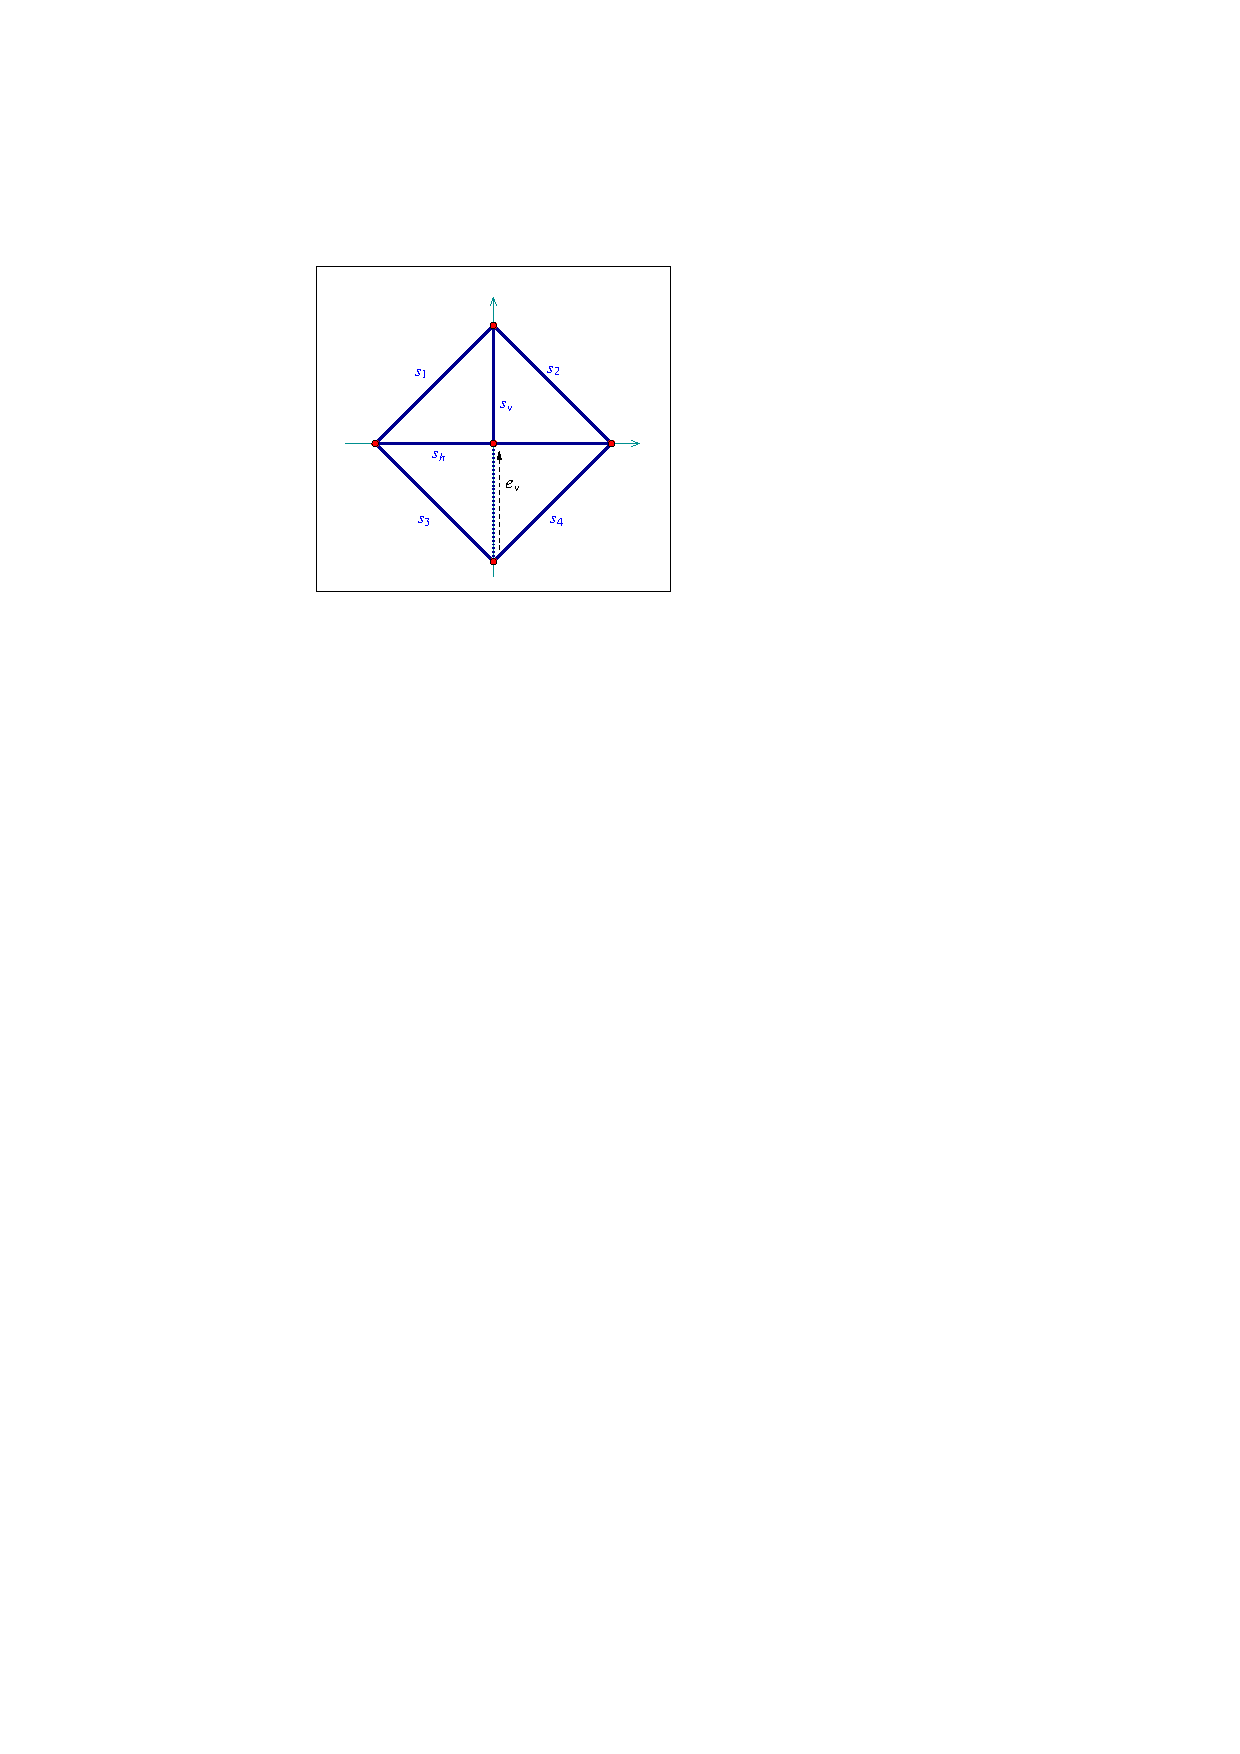
\includegraphics{Arrangement_2/fig/ex_19}
  \end{center}
\end{ccTexOnly}
\begin{ccHtmlOnly}
  <p><center>
  <img src="./fig/ex_19.gif" border=0 alt="Example 19">
  </center>
\end{ccHtmlOnly}
\caption{An arrangement of five line segments, as constructed in
\ccc{ex_observer.C}. The halfedge $e_v$ (dashed) is eventually
removed, so that the final arrangement consists of four faces (one
unbounded and three bounded ones).\label{arr_fig:ex_19}}
\end{figure}

The following example shows how to define and use an observer
class. The observer in the example keeps track of the arrangement
faces, and prints a message whenever a face is split into two due
to the insertion of an edge, and whenever two faces merge into one
due to the removal of an edge. The layout of the arrangement is
depicted in Figure~\ref{arr_fig:ex_19}:

\ccIncludeExampleCode{../examples/Arrangement_2/ex_observer.C}

Observers are especially useful when the \dcel\ records are
extended and store additional data, as they help updating this
data on-line. See Section~\ref{arr_sec:ex_dcel} for more details
and examples.
